
\title{Recap System and device programming (01NYHOV)}
\author{Jacopo Nasi\\
        Computer Engineer\\
        Politecnico di Torino}
\date{II Period - 2017/2018\\\bigskip\bigskip\today}

\documentclass[12pt]{article}
\usepackage[utf8]{inputenc}
\usepackage[italian]{babel}
\usepackage{geometry}
\usepackage{indentfirst} % First line indent
\usepackage{mathtools}
\usepackage{wrapfig}
\usepackage[usenames, dvipsnames]{color}
\usepackage{float}
\usepackage{amssymb}
\usepackage{ifsym}


% Misure Documento
\geometry{ a4paper, total={170mm,257mm},left=35mm, right=35mm, top=35mm, bottom=35mm }

\begin{document}

\begin{figure}
  \centering
  
\includegraphics[width=10cm]{images/polito.pdf}
\end{figure}

\maketitle

\newpage
\tableofcontents

\newpage
{\noindent \Large \textbf{License}\bigskip}

This work is licensed under a Creative Commons Attribution-NonCommercial-ShareAlike 3.0 Unported License.\\
You are free:
\begin{itemize}
  \item \textbf{to Share}: to copy, distribute and transmit the work
  \item \textbf{to Remix}: to adapt the work
\end{itemize}
Under the following conditions:
\begin{itemize}
  \item \textbf{Attribution}: you must attribute the work in the manner specified by the author or licensor (but not in any way that suggests that they endorse you or your use of the work)
  \item \textbf{Noncommercial}: you may not use this work for commercial purposes.
  \item \textbf{Share Alike}: if you alter, transform, or build upon this work, you may distribute the resulting work only under the same or similar license to this one.
\end{itemize}

\noindent More information on the Creative Commons website (http://creativecommons.org).

\begin{figure}[h!]
  \centering
  
\includegraphics[width=3cm]{images/license.png}
\end{figure}

{\noindent \Large \textbf{Acknowledgments}\bigskip}

Questo breve riepilogo non ha alcuno scopo se non quello di agevolare lo studio di me stesso, se vi fosse di aiuto siete liberi di usarlo.\\
Le fonti su cui mi sono basato sono quelle relative al corso offerto (\textbf{System and device programming (01NYHOV)}) dal Politecnico di Torino durante l'anno accademico 2017/2018.\\
Non mi assumo nessuna responsabilità in merito ad errori o qualsiasi altra cosa. Fatene buon uso!
\newpage


\section{Review}
\subsection{Processes}
An \textbf{Algorithm} is a logical procedure that in a finite number of steps solves problem. A \textbf{Program} is a formal expression of an algorithm by means of a programming language. The \textbf{Process} is a sequence of operations performed by a program in execution on a given set of input data. The structure of a process, figure \ref{fig:proc_mem} is made by:
\begin{itemize}
  \item Text area (source code)
  \item Data Area (global variables)
  \item Stack (functions parameters and local variables)
  \item Heap (dynamic variables allocated during the process execution)
  \item Registers (program counter, stack pointer, ecc...)
\end{itemize}
\begin{figure}[H]
  \centering
  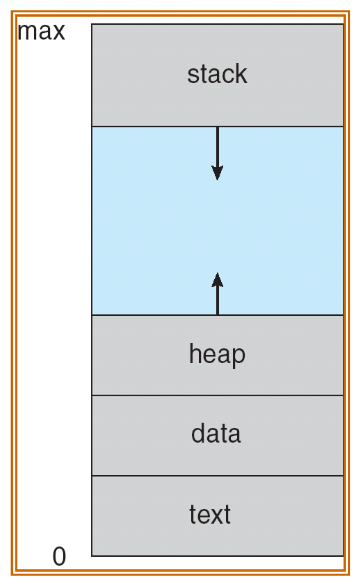
\includegraphics[width=0.5\linewidth]{images/proc_mem.png}
  \caption{Process memory layout}
  \label{fig:proc_mem}
\end{figure}
The trace of a process is its entire line, it represent the state at any time. An important operation is the possibility to freeze the state of a process in order to execute other tasks. This choice is demanded to the CPU scheduler. The possibility to switch from a state sto another is called \textbf{Context Switching}.\\
Each processes has a unique (while the process is active) identifier (\textbf{PID}), a positive integer.\\
The \textbf{\textit{fork()}} is the system call used to create a new child process. The child is a copy of the parent execluding the Processs ID returned by the fork.
\begin{itemize}
  \item The parent process receives the child PIDs.
  \item The child process receives the value 0.
\end{itemize}
The 2 processes are perfect clones with 2 different heap, 2 stacks, etc... The only shared part is the code. A process can become orphan if the parent dies, in that case is become son of the INIT process (PID: 1). Another possible state is the zombie, where the process has terminated its execution but still has an entry in the process state. The zombie state waste resources and must be avoided. During the fork process the child inherit the value of local variable from the parent but they are different varible and they aren't linked, the address space of the 2 processes is different.
There are several way to exit from a process:
\begin{itemize}
  \item \textit{return}
  \item \textit{exit}
\end{itemize}
there are also other not correct termination, like \textit{abort}. The correct behaviour require that the parent \textbf{\textit{wait()}} for the process terminations of tis sons, the kernel sends a signal (\textbf{SIDCHLD}) to its parent. The parent can manage or ignore it.\\
The system call \textbf{\textit{exec()}} is different from the fork because it run a different executable, it does not create another process, it substitutes the calling process image with the image of another program.

\subsection{Operating System}
The OS is not a program, is a set of modules, a big interrupt routine. It reacts to action like mouse moving, ecc... The user can't exxecute all the instriction set. The CPU runs in at least 2 states (mode):
\begin{itemize}
  \item Kernel
  \item User
\end{itemize}
Each mode defined different access rights, of course the kernel mode is the most powerfull. The are some instruction that are priviledged, like the I\/O, or over some registers due to concurrency where the controll is CPU demanded.\\
\subsection{Kernel}
The kernel is a black box, the only way to interact with it is to used the interrupts provided. By receiving and address the kernel know that it must perform, for example, a reading operation and so on. Is not possible to access directly to the kernel memory.

\subsection{Shell}
The shell is not part of the kernel, is like all other processes. The user perform, through it, system calls that run at the user level.

\subsection{Threads}
The process are really "exprensive" in case of cooperation, the clone operation involves a significant increase of memory used and the creation time become an overhead. Also the context switching can become expensive. A possible solution to all these problem is using \textbf{threads}. For the kernel different threads are part os a single process. The context switch is really faster because the context "is the same". The process is the owner of the resources that are used by all its threads. The thread is the basic unit of CPU utilization (and scheduling). They are also called lightweight processes.
\begin{figure}[H]
  \centering
  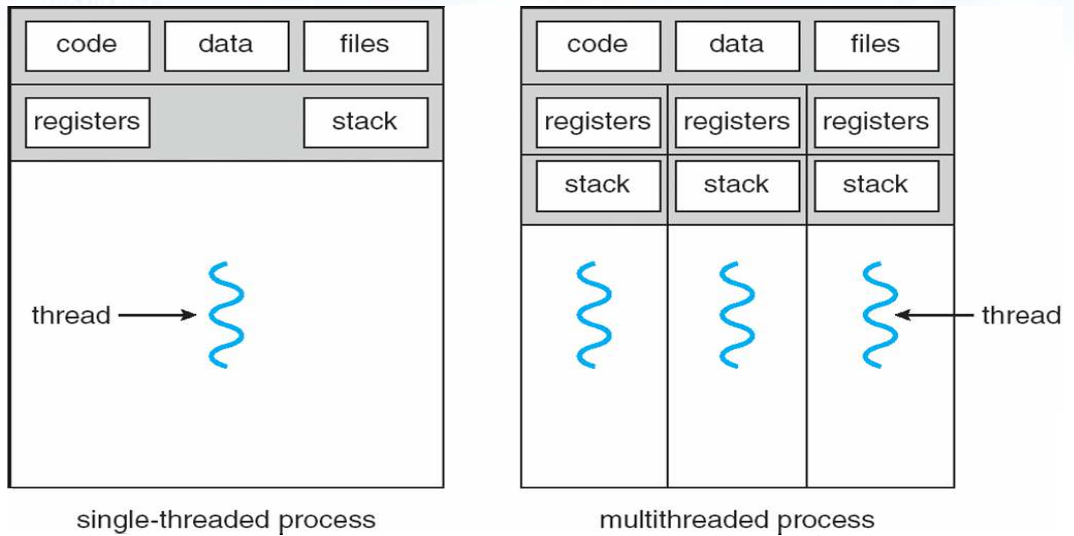
\includegraphics[width=0.5\linewidth]{images/proc_thread.png}
  \caption{Processes and Threads}
  \label{fig:proc_thread}
\end{figure}

\subsection{Critical section}
Also know as Critical Region, is a section of code, common to multiple threads, in which they can access (read and write) shared objects. A section in which threads are competing for the use (R\/W) of shared resources. We want to ensure that when one thread is executing in its CS, no other thread is allowed to execute in its CS. THe solution is to establish an access protocol to enter the critical section in \textbf{mutual exclusion}.\\
There are different solutions to solve this problem:
\begin{itemize}
  \item software
  \item hardware
  \item System Call (semaphore)
\end{itemize}

\subsection{Semaphore}
System call used to manage critical sections and to solve synchronization problem. The semaphore primitives allows thread to:
\begin{itemize}
  \item Create semaphore (init)
  \item Be blocked on the semaphore (wait)
  \item Wakeup if it was blocked (signal)
  \item Destroy a sempahore (destroy)
\end{itemize}
The operations on a semaphore are \textbf{ATOMIC}, it is impossible for two threads to perform simultaneously operations on the same semaphore.\\
Another type of semaphore is the MUTEX, or binary semaphore, they are a little bit easier to be managed but they are less powerfull. Only the action lock and unlock must be performed.\\
Sempahores can be also implemented like pipes.

\section{Memory Management}
Chapter about hardware memory organization, discussing MM techniques like paging and segementation.

\subsection{Background}
A program must be brought (from disk) into main memory and placed within a process for it to be run. Main memory and registers are onyl CPU storage and only it can access directly to them. The register access is performed in one CPU clock, the main memory could require more cycles, the cache instead is between them (speed speaking).\\
The address binding of instructions and data to memory addresses can happen at three different stages:
\begin{itemize}
  \item \textbf{Compile Time}: If memory location know a priori, absolute code can be generated; must recompile code if starting location changes.
  \item \textbf{Load Time}: Must generate relocatable code if memory location is not know at compile time.
  \item \textbf{Execution Time}: Binding delayed until run time if the process can be moved during its execution from one memory segment to another. Need hardware support for address maps. (e.g. base and limit register)
\end{itemize}
\begin{figure}[H]
  \centering
  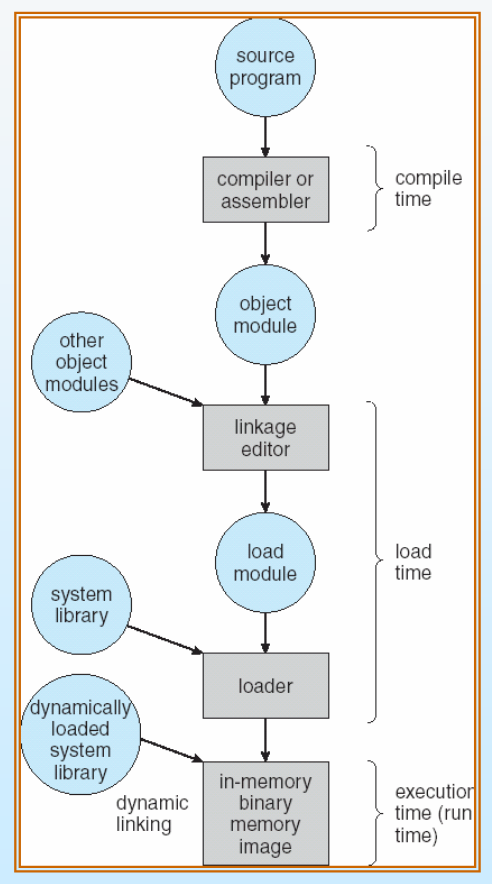
\includegraphics[width=0.4\linewidth]{images/multi_step_user.png}
  \caption{Multistep processing of a user program}
  \label{fig:multi_step_user}
\end{figure}

The concept of a logical addresses space that is bound to a separta physical address space is central to proper memory management.
\begin{itemize}
  \item \textbf{Logical}: Generated by the CPU; also referred as \textbf{virtual addresses}.
  \item \textbf{Physical}: Address seen by the memory unit.
\end{itemize}
Logical and physical addresses are the same in compile-time and load-time address-binding schemes; logical (virtual) and physical addresses differ in execution-time address-binding scheme.\\
The \textbf{MMU} (\textit{Memory-Management Unit}) is an hardware device that maps virtual to physical address. In its scheme, the value in the relocation register is added to every address generated by a user process at the time it is sent to memory. Every user program deals only with logical addresses.\\
Using the \textbf{Dynamic Loading} routine is not loaded until it is called, this allows a better memory space utilization (unused routine is never loaded). This function is useful when large amounts of code are needed to handle infrequently occuring cases.\\
Another important mechanism is the \textbf{Dynamic Linking} where the linking is postponed until execution time. Small piece of code, \textit{stub}, used to locate the appropriate memory-resident library routine, replaces itself with the address of the routine, and executes the routine. OS needed to check if routine is in processes memory addresses. This solution is particularly useful for libraries. It is also know as \textbf{Shared Libraries}.

\subsection{Swapping}
A process can be swapped temporarily out of memory to a backing store, and then brought back into memory for continued execution.\\
\textbf{Backing Store} fast disk large enough to accommodate copies of all memory images for all users; must provide direct access to these memory images. \textbf{Roll out, Roll in} swapping variant used for priority-based scheduling algorithms; lower-priority process is swapped out so higher-priority process can be loaded and executed.\\
The greatest part of swap time is spent in transfer time; total transfer time is directly proportional to the amount of memory swapped. Each system maintains a ready queue of ready-to-run processes which have memory images on disk. AN example of swapping in figure \ref{fig:swap}.
\begin{figure}[H]
  \centering
  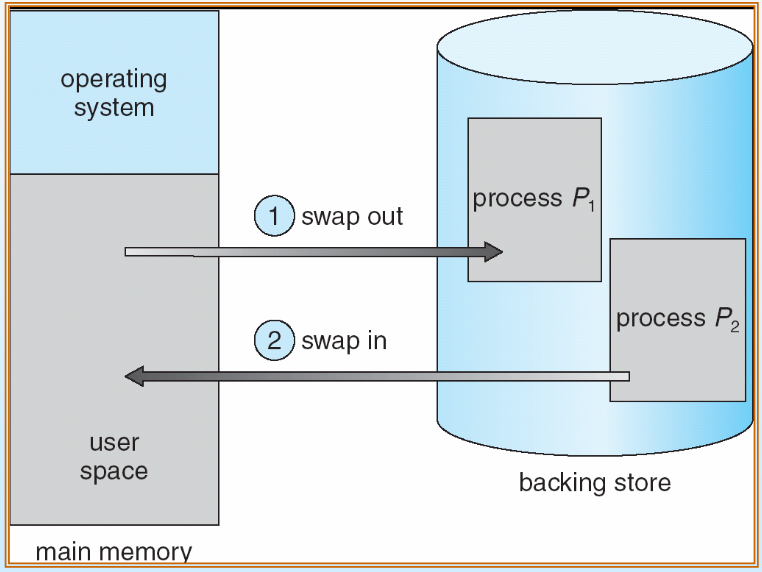
\includegraphics[width=0.4\linewidth]{images/swap.png}
  \caption{Swapping process}
  \label{fig:swap}
\end{figure}

\subsection{Contigous Allocation}
Main memory is usually into two parts:
\begin{itemize}
  \item Resident OS, usually held in low memory with interrupt vector.
  \item Use processes in the high part.
\end{itemize}
Relocation registers used to protect user processes from each other, and from changing OS code and data:
\begin{itemize}
  \item Base register contains value of smallest physical addresses.
  \item Limit register contains range of logical addresses must be less than the limit register.
  \item MMU maps logical address \textit{dynamically}.
\end{itemize}

Multiple-partition allocation is based on \textbf{Hole}: block of available memory; holes of various size are scattered throughout memory. When the process arrives, it is allocated memory from a hole large enough to accommodate it. The OS maintains information about:
\begin{itemize}
  \item Allocated Partitions
  \item Free Partitions (hole)
\end{itemize}

\subsection{Dynamic Storage-Allocation Problem}
There are several solution to how satisfy a request of size \textit{n} from a list of free holes:
\begin{itemize}
  \item \textbf{First-fit}: Allocate the \textit{first} hole that is big enough.
  \item \textbf{Best-fit}: Allocate the \textit{smallest} hole that is big enough; must search entire list (unless ordered by size). It produces the smallest leftover hole.
  \item \textbf{Worst-fit}: Allocate the \textit{largest} hole; must also search the entire list. It produces the largest leftover hole.
\end{itemize}
First and best fit are better than worst in terms of speed and storage utilization.

\subsection{Fragmentation}
The \textbf{External} is the total memory exists to satisfy a request, but it is not contiguous. The \textbf{Internal} instead is the allocated memory that can be slightly larger that requested memory; this size difference is memory internal to a partition, but not being used.\\
Is possible to reduce the fragmentation by using the \textbf{compaction}. Shuffle memory contents to place all free memory together in one large block. Compation is possible only is the relocation is dynamic, and is done at execution time. There are some I\/O problems:
\begin{itemize}
  \item Latch job in memory while it is involved in I\/O.
  \item Do I\/O only into OS buffers.
\end{itemize}

\subsection{Paging}
The paging is a memory management scheme by which a computer stores and retrieves data from secondary storage for use in main memory.\\
Logical address space of a process can be non-contiguous; process is allocated in physical memory whenever the latter is available. Divide physical memory into fixed-sized blocks called \textbf{frames} (size power of 2, between 512 bytes and 8'192 bytes) and keep track of all of them. Divide logical memory into blocks of same size called \textbf{pages}. When a program of \textit{n} pages need to be runned, all the \textit{n} frames must be finded and loaded. Using this solution is important to set up a page table to translate logical to physical addresses. These process of course incurs in internal fragmentation.\\
\paragraph{Address Translation Scheme} divide the addresses generated by the CPU into:
\begin{itemize}
  \item \textbf{Page Number (p)}: Used as an index into a page table which contains base address of each page in physical memory.
  \item \textbf{Page Offset (d)}: Combined with base address to define the physical address that is sent to the memory unit.
\end{itemize}
\begin{center}
  \begin{tabular}{ |c|c| }
    \hline
    \textbf{Page Number} & \textbf{Page Offset}\\
    \hline
    p & d\\
    \hline
    m - n & n\\
    \hline
  \end{tabular}
\end{center}
\begin{figure}[H]
  \centering
  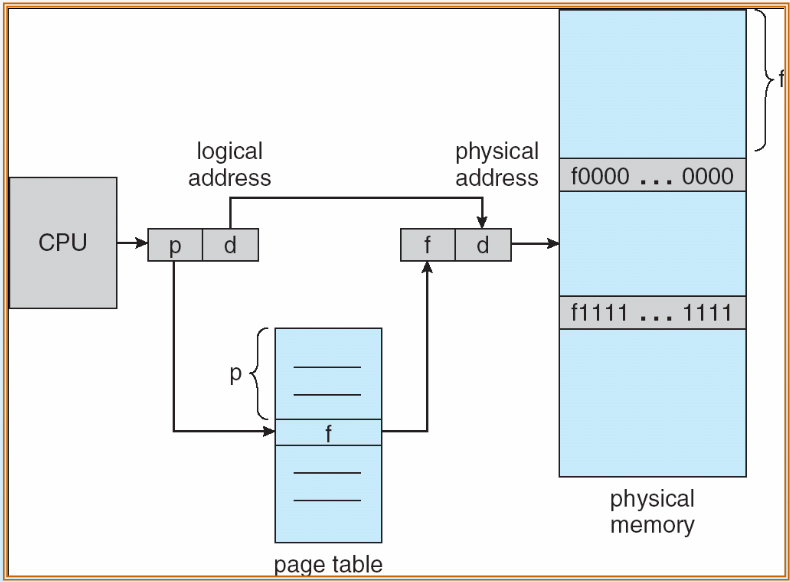
\includegraphics[width=0.8\linewidth]{images/paging.png}
  \caption{Paging Hardware}
  \label{fig:paging}
\end{figure}
\begin{figure}[h]
  \centering
  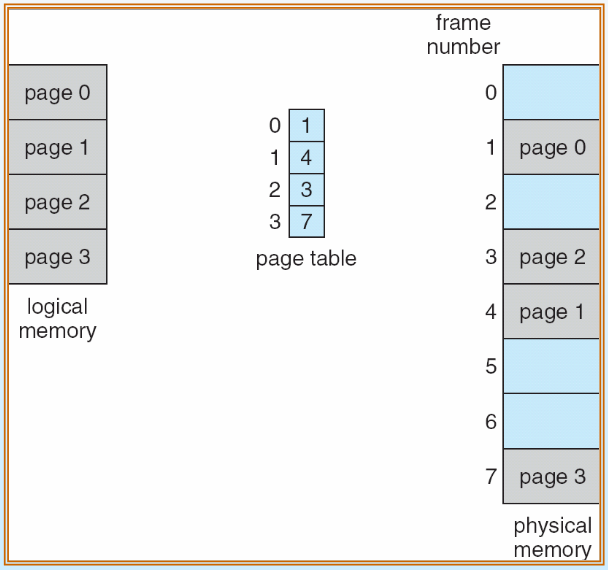
\includegraphics[width=0.8\linewidth]{images/ex_paging.png}
  \caption{Paging Example}
  \label{fig:ex_paging}
\end{figure}

\paragraph{Page Table} is kept in main memory, it can be of 2 types:
\begin{itemize}
  \item \textbf{PTBR} (Base Register): Points to the page table.
  \item \textbf{PRLR} (Lenght Register): Indicates size of the page table.
\end{itemize}
In this scheme every data/instruction access requires two memory accesses. One for the page table and one for the data/instruction. This double-access problem can be solved by the use of a special fast-lookup hardware cache called \textbf{Associative Memory} or \textbf{Translation Look-aside Buffers} (TLBs). Some TLBs soter address-space identifiers (ASIDs) in each TLB entry: uniquely identifies each process to provide address-space protection for that process.\\
In all cases the \textbf{Effective Access Time} (EAT) is computed:
\begin{equation} \label{eat}
  EAT = (t + \epsilon)*\alpha + (2*t + \epsilon)(1 - \alpha)
\end{equation}
where:
\begin{itemize}
  \item $\epsilon$: Associative lookup time unit
  \item t: Memory cycle time
  \item $\alpha$: Hit ratio
\end{itemize}

\subsection{Memory Protection}
The MP is implemented by associating protection bit with each frame. \textbf{Valid-Invialid} (means "if is in the code domain") bit attached to each entry in the page table:
\begin{itemize}
  \item \textbf{Valid}: Indicate that the associated page is in the process logical address space, and is thus a legal page.
  \item \textbf{Invalid}: Indicates that the page is not in the process logical address space.
\end{itemize}

\subsection{Shared Pages}
The \textbf{shared code} is one copy of read-only (reentrant) code shared among processes (i.e., text editors, compilers, window system). Shared code must appear in same locaiton in the logical address space of all processes. Regarding \textbf{private code and data}, each process keeps a separate copy of them. The pages for the private code and data can appear anywhere in the logical address space.

\begin{figure}[h]
  \centering
  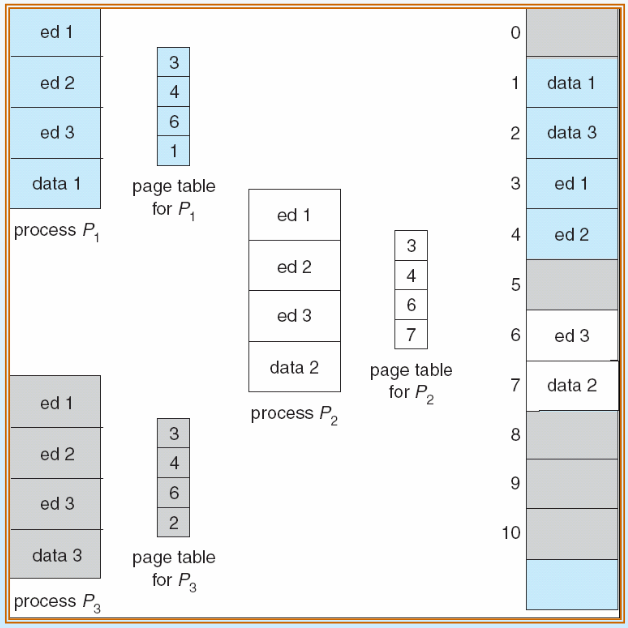
\includegraphics[width=0.8\linewidth]{images/shared_page.png}
  \caption{Shared Page}
  \label{fig:shared_page}
\end{figure}

\subsection{Page Table}
They can be of 3 types:
\begin{itemize}
  \item \textbf{Hierarchical}
  \item \textbf{Hashed}
  \item \textbf{Inverted}
\end{itemize}
the choice is related to the page size.\\
The first one, the \textbf{hirearchical}, breaks the logical address space into multiple page tables, a simple technique is a two-level page table. This solution is not actuable in 64-bit system.
A possible example with a Two-Level pagin could be:
\begin{itemize}
  \item \textbf{Page Number} consisting of 22-bit: (since is paged is further divided)
  \begin{itemize}
    \item 12-bit page number
    \item 10-bit offset
  \end{itemize}
  \item \textbf{Page Offset} consisting of 10-bit
\end{itemize}
Thus the logical address is as follows:
\begin{center}
  \begin{tabular}{ |c|c|c| }
    \hline
    \multicolumn{2}{|c|}{\textbf{Page Number}} & \textbf{Page Offset}\\
    \hline
    $p_i$ & $p_2$ & d\\
    \hline
    12 & 10 & 10\\
    \hline
  \end{tabular}
\end{center}
A 3-level architecture is used in order to correctly and completely addressing 64-bit addresses.\\
The \textbf{hashed} architecture is common in address spaces greater than 32 bit. The virtual page is hashed into a page table. This page table contains a chain of elements hashing to the same location. Virtual page numbers are compared in this chain searching for a match. If a match is found, the corrisponding physical fram is extracted.\\
The last type, \textbf{inverted}, has one entry for each real page of memory. Entry consist of the virtual address of the page stored in that real memory location, with the information about the process that owns that page. Decreases memory needed to store each page table, but increases time needed to search the table when a page reference occurs. This last solution is affordable only with few memory of course.

\subsection{Segmentation}
MM scheme that supports user view of memory. A program is a collection of segments. The segment is a logical unit such as:
\begin{itemize}
  \item main program \item procedure \item function
\end{itemize}
The difference respect the page is that, the page, has a fixed size and it's a memory region. The segmente instead is variable.\\
\paragraph{Architecture} the logical address consists of two tuple: $<$segmentNumber$, $offset$>$. The segment table maps two-dimensional physical address; each table entry has:
\begin{itemize}
  \item \textbf{Base}: Contatins the starting physical address where the segments reside in memory.
  \item \textbf{Limit}: Specifies the length of the segment.
\end{itemize}
There are also other 2 important values:
\begin{itemize}
  \item \textbf{STBR} (Segment-Table Base Register): Points to the segment table's location in memory.
  \item \textbf{STLR} (Segment-Table Length Register): Indicates number of segments used by a program.
\end{itemize}
This means that the segment number \textit{s} is legal only if (s$<$STLR).\\
This solution implements also some protection mechanisms. For each entry in the segment table is asociated a:
\begin{itemize}
  \item Validation bit = 0 (illegal segment)
  \item read/write/execute privileges
\end{itemize}
Protection bits is associated with segments, code sharing occcurs at segment level. Since segments vary in length, memory allocation is a dynamic storage-allocation problem.

\section{Virtual Memory}
Benefits of VMS, demand paging, page-replacemement and allocation of page frames.

\subsection{Background}
The \textbf{Virtual Memory} is the separation of user logical memory from physical memory.
\begin{itemize}
  \item Only parte of the program needs to be in memory for the execution.
  \item Logical address space can therefor be much larger than physical address space.
  \item Allows address spaces to be shared by several processes.
  \item Allows for more efficent process creation.
\end{itemize}
The virtual memory of course offer bettere characteristics than the hardware one. It can be implemented via: \textbf{Demand Paging} and \textbf{Demand Segmentation}.

\subsection{Demand Paging}
This solution bring page into memory only when it is needed. This implies a lot of benefit. Less I/O, less memory needed, faster response, more users.\\
When a page is needed the reference to it is computed, if the reference is invalid $\Rightarrow$ abort, if the page isn't in memory $\Rightarrow$ bring to memory. The main idea is to implement a \textbf{Lazy swapper} that never swap page into memory unlesse page will be needed, the swapper is also called \textbf{pager}.
\begin{figure}[h]
  \centering
  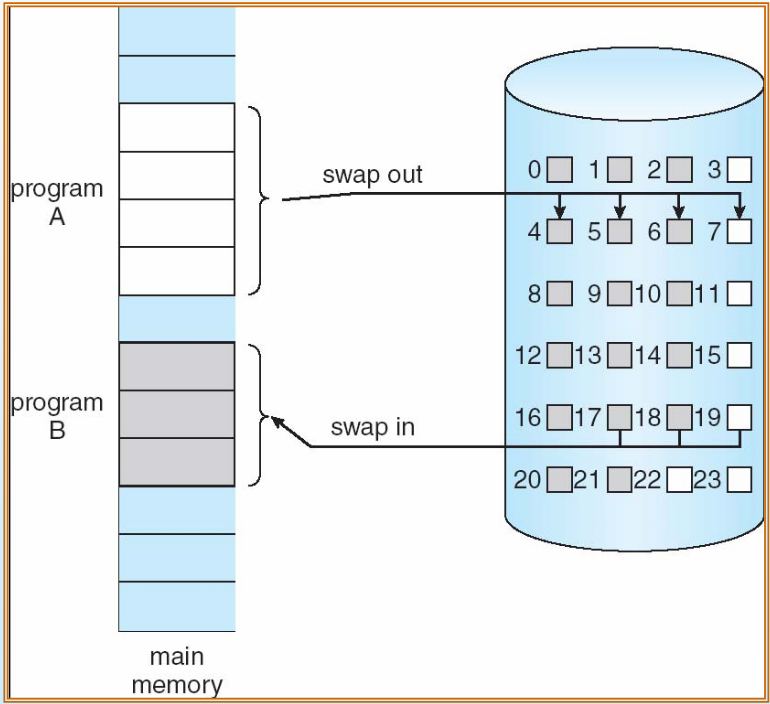
\includegraphics[width=0.8\linewidth]{images/swapping.png}
  \caption{Swapping of memory}
  \label{fig:swapping}
\end{figure}

\paragraph{Valid-Invalid Bit} with each page table entry a valid-invalid bit is accociated, it means that \textbf{Valid = In Memory}, \textbf{Invalid = Not in Memory}.

\subsection{Page Fault}
If there is a reference to a page, and if that page is not already in memory, first reference to that page will trap to operating system: Page Fault. The flow is the following:
\begin{enumerate}
  \item OS look to anothe rtable to decide:
  \begin{itemize}
    \item Invalid reference = abort
    \item Just not in Memory = continue
  \end{itemize}
  \item Get empty frame
  \item Swap page into frames
  \item Reset tables
  \item Set validation bit = V
  \item Restart the instruction that caused the page fault
\end{enumerate}

\subsection{Process creation}
The use of virtual memory allows other benefits during process creation:
\paragraph{Copy-on-write} it allows both parent and child process to initially share the same pages in memory. If eother process modifies a shared page, only then is the page copied. This solution allows more efficient process creation as only modified pages are copied. Free pages are allocated from a pool of zerod-out pages. If there is not free frame page replacement is performed.\\
\paragraph{Page Replacement} prevent over-allocation of memory by modifing page-fault service routine to include page replacement. Use modify (dirty) bit to reduce overhead of page transfers - only modified pages are written to disk.
Page replacemente completes separation between logical memory and physical memory - large virtual memory can be provided on a smaller physical memory. The basic flow of page replacement is the following:
\begin{itemize}
  \item Find location of the desired page on disk
  \item Find a free frame:
  \begin{itemize}
    \item If there is a free frame = Use it
    \item If there is not a free frame = Use page replacement to select victim
  \end{itemize}
  \item Bring the desired page into the new free frame, update the page and frames table
  \item Restart process
\end{itemize}
There are several algorithms that can be used in order to perform page replacement:
\begin{itemize}
  \item \textbf{FIFO}: The oldest page is the first replaced.
  \item \textbf{LRU}: Replace the page that will not be used for the longest period of time.
  \item \textbf{LFU}: Replace page with the smallest count of usage.
  \item \textbf{MFU}: The page with the smallest count is just be brought in and has yet to be used.
\end{itemize}

\subsection{Memory-mapped files}
Memory-mapped file I\/O allows file I\/O to be trated as routine memory access by mapping a disk block to a page in memory. A file is initially read using demand paging. A page-sized portion of the file is read from the file system into a physical page. Subsequent reads\/write to\/from the file are treated as ordinary memory accesses. This allows a simplified acces through memory rather than read() of write() operations. It can be also used to shared file among different processes.

\subsection{Kernel Memory}
Treated differently from user memory. Often allocated from a free-memory pool:
\begin{itemize}
  \item Kernel requests memory for structures of varying sizes.
  \item Some kernel memory needs to be contiguous.
\end{itemize}
\paragraph{Buddy system} allocates memory from fixed-size segement consisting of physically-contiguous pages. The memory is allocated using \textbf{power-of-2 allocator}.
\paragraph{Slab Allocator} it alternate strategy, slab is one or more physically contiguos pages. Cache consists of one or more slabs. Single cache for each unique kernel data structure.
% END OF CHAPTER 9 - mm2-ch9.pdf
% STARTING IO.pdf
\section{I\/O}
This chapter will speak about Unix kernel architecture, file system data structure, etc...

\subsection{Kernel}
The kernel architecture is represented in figure \ref{fig:unixkernel}.
\begin{figure}[h]
  \centering
  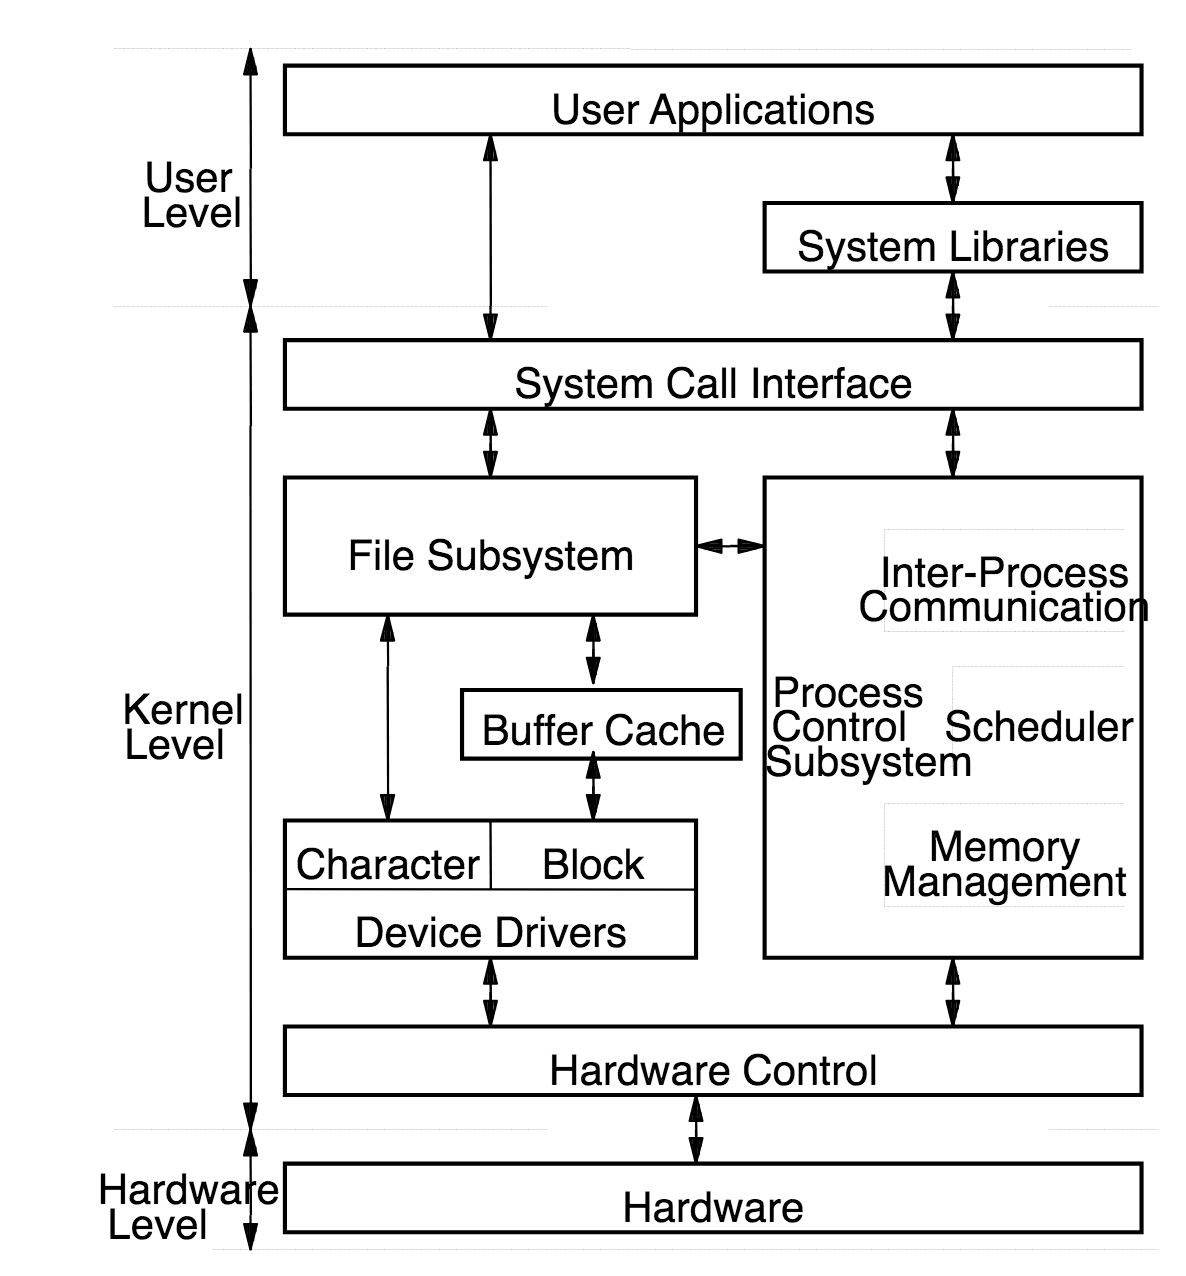
\includegraphics[width=0.8\linewidth]{images/unixkernel.png}
  \caption{UNIX Kernel architecture}
  \label{fig:unixkernel}
\end{figure}
Is divided in 3 levels:
\begin{enumerate}
  \item Hardware
  \item Kernel
  \item User
\end{enumerate}

\subsection{Terminal Driver}
Include one or more line discipline modules, which interpret the input chars and format the output lines. Every disciplined line may operate in two modes:
\begin{itemize}
  \item \textbf{Raw mode}: The line discipline transfers data between a terminal and a process without any conversion.
  \item \textbf{Canonical mode}: The user input is converted for the receiving process. The process output is converted for the user.
\end{itemize}

\subsection{Buffer cache}
When the kernel is asked to serve a read request from disk it tries to read the data from the buffer cache. If the data are in the cache, they will returned to the user process without any disk access. Otherwise, the kernel, reads a block of data from disk and stores it in the buffer cache, trying to keep it in memory as long as possible, for a possible future usage.\\
When the kernel is asked to server a write request to disk, it puts the data in the buffer cache:
\begin{itemize}
  \item Data stay in memory for possible read operations.
  \item Addition or change of the data are performed in memory rather than disk.
\end{itemize}
The goal of the buffer cache is trying to minimize the number of disk accesses:
\begin{itemize}
  \item By reading ahead the data that, according to the space and temporal locality of the process references, have high probability to be referenced in the near future.
  \item By delaying as much as possible the transfer of the contente of the buffer cache to disk ()\textbf{dealyed write}.)
\end{itemize}

\section{Booting a PC}
The booting process is not easy. The first PCs, were based on the 16-bit Intel 8088 processor that were only capable of addressing 1MB of physical memory. The physycal address space of an early PC would therefore start at 0x00000000 but end at 0x000FFFFF instead of 0xFFFFFFFF. The 640KB are marked "low memory" was the only RAM that an early PC could use. Figure \ref{fig:memory8088}.
\begin{figure}[h]
  \centering
  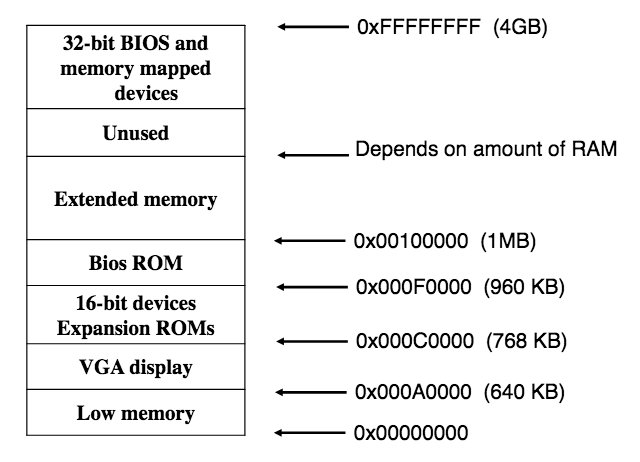
\includegraphics[width=0.8\linewidth]{images/memory8088.png}
  \caption{Memory view of 8088 processor}
  \label{fig:memory8088}
\end{figure}
The 348KB area from 0x000A0000 through 0x000FFFFF was reserved by the hardware for special uses such as video display buffers and firmware held in nonvolatile memory. The most important part of this reserved are is the basic Input\/Output System (BIOS), which occupies 64KB.

\subsection{BIOS}
More BIOS is located at the high end of the 32-bit address range for user by 32bit PCI devices. The BIOS is responsible for performing Power-On-Self-Test and basic system initialization such as activating the video card and checking the amount of memory installed. After performing this initialization, the BIOS loads the OS from some appropriate location such as floppy disk, HDD, CD-ROM or Network and passes control of the machine to the OS.

\subsection{ROM BIOS}
The 486 and later processors start executing at physycal address 0xFFFFFFF0, which is at the very top of the memory space, in an are reserved for the ROM BIOS. The first instruction is:
\begin{itemize}
  \item [] JMP FAR f000:e05b
\end{itemize}
This instruction jumps to the normal BIOS, which is located in the 64KB region from 0xF0000 to 0xFFFFF mentioned above.
The CPU start in real mode, so the \textit{JMP FAR} instriction is a real mode jump that restoers us to low memory. In real mode, the segmented address segment:offset translates to the physical address segment*16+offset. Thus, f00:e05b traslates to 0x000fe05b.\\
No GDT, LDT or paging table is needed by the CPU in real mode. The code that initializes these data structures must run in real mode. When the BIOS runs:
\begin{itemize}
  \item It initializes the PCI bus and all the important devices it knows about (in particular VGA display).
  \item Then it searches for a bootable devices such as a floppy, HDD, etc...
  \item When it finds a bootable disk, it reads the boot loader from the disk and transfers control to it.
\end{itemize}

\subsection{BOOT Loader}
Is the program run by the BISO to load the image of a kernle into RAM. Floppy and companies for PCs are, by historical convention, divided up into 512 byte regions called sectors. If the disk is bootable, the first sector is called boot sector, since this is where the boot loader code resides. When the BIOS finds a bootable floppy or HDD, it loads the 512 byte boot sector into low memory, at physical addresses: 0x7C00 through 0x7DFF. Then uses a JMP instruction to set the CS:IP to 0000:7C00, passing control to the boot loader.
\paragraph{Files} The boot loader user three main files:
\begin{itemize}
  \item \textit{\textbf{boot.s}}: First the boot loader switches the processor from real mode to 32-bit protected mode, because is the only mode that software can access all the memory above 1MB inh physical address space.
  \item \textit{\textbf{main.c}}: Second, the boot loader reads the kernel from the HDD by directly accessing the IDE disk device registers via the x86's special I\/O instructions.
  \item \textit{\textbf{boot.asm}}: This file is a disassembly of the boot loader. It is easy to see exactly where in physical memory all of the boot loader's code resides.
\end{itemize}
\paragraph{Passing control to Kernel} The boot loader's link and load addresses match perfectly. There is a rather large disparty between the kernel's link and the load addresses. Operating system kernels often like to be linked and run at very high virtual address in order to leave the lower part of the processor virtual address space for user programs to use.

\subsection{Kernel load address and virtual addresses}
Since we can't actually load the kernel at physical address 0xf0100000, we will use the processor's memory management hardware to map vistual address to the physical, where the boot loader actually load the kernel.
% FINISH BOOTING_PC.pdf














\end{document}
